\subsection{Hash Tables}
    \begin{minipage}{0.49\linewidth}
        \begin{itemize}
            \item fast access to elements
            \item Unsorted, unordered data
            \item $\mathcal(O)$ only in expectation
        \end{itemize}
        Given an element 'x' to be stored, a Hash Table 'M' of length 'l' and a hash function 'f(x)':
        \begin{lstlisting}
M[f(x) % l] = x
\end{lstlisting}
    \end{minipage}
    \begin{minipage}{0.49\linewidth}
        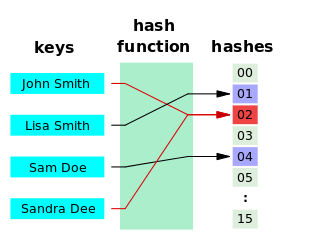
\includegraphics[width = 0.95\linewidth]{src/5_data_structure/images/hash_function.png}
        \textcolor{red}{example of collision}
    \end{minipage}

    \subsubsection{Collision handling}
        Entry at calculated index may already contain an element
        \begin{tabular}{p{0.45\linewidth} | p{0.45\linewidth}}
            \hline
            Probing: next available index is chosen & Chaining: a linked list at every entry\\
            \hline
            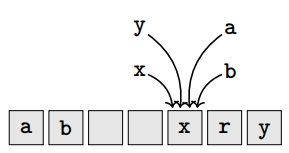
\includegraphics[width = \linewidth]{src/5_data_structure/images/probing.png} & 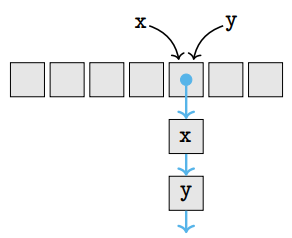
\includegraphics[width = \linewidth]{src/5_data_structure/images/chaining.png}
        \end{tabular}
